% !TEX TS-program = arara
% arara: clean: {files: [ elaborat.aux, elaborat.bbl, elaborat.toc]}
% arara: xelatex
% arara: nomencl
% arara: biber
% arara: biber
% arara: xelatex
% arara: xelatex
% arara: clean: {files: [elaborat.aux, elaborat.bbl, elaborat.toc, elaborat.nls, elaborat.nlo, elaborat.ilg, elaborat.bcf, elaborat.blg, elaborat.out, elaborat.run.xml, elaborat.lof]}
%
%
%
% tex essentials
\documentclass[german,12pt,oneside,titlepage,listof=totoc,bibliography=totoc]{scrartcl}
\usepackage[a4paper, left=4cm, right=2cm, top=4cm, bottom=2cm]{geometry}
\usepackage[automark,plainheadsepline,singlespacing=true]{scrlayer-scrpage}
	\pagestyle{scrheadings}\clearpairofpagestyles
	\chead{\Roman{page}}\setkomafont{pageheadfoot}{\normalfont}\pagenumbering{Roman}
\usepackage{blindtext}
\usepackage{mdwlist}
\usepackage{hvfloat}
\usepackage{caption}
	\captionsetup[figure]{%
		labelfont={bf,rm},
		textfont={bf,rm},
		justification=raggedright,
		singlelinecheck=off
	}
	\captionsetup[table]{%
		labelfont={bf,rm},
		textfont={bf,rm},
		justification=raggedright,
		singlelinecheck=off
	}
	\newcommand{\capquelle}[1]{%
		\par\parbox{\captionwidth}{\raggedright\bigskip Quelle: #1}%
	}

% text Language
\usepackage[german=quotes,autostyle]{csquotes}
\usepackage[ngerman]{babel}
\usepackage[T1]{fontenc}
\usepackage{setspace}

% toc Appendix
\usepackage[intoc]{nomencl}
\usepackage{appendix}
\usepackage{pdfpages}
\usepackage[printonlyused]{acronym}

% Font
\usepackage{newtxmath}
\usepackage{fontspec}
\usepackage{anyfontsize}
	\setmainfont{Times New Roman}
	\defaultfontfeatures[\rmfamily,\sffamily]{Ligatures=TeX}
	\addtokomafont{sectionentry}{\mdseries}
	\setkomafont{sectioning}{\bfseries}

% bibliography
\usepackage[backend=biber,style=ext-authoryear,maxcitenames=1,maxbibnames=999,mergedate=false,date=iso,seconds=true,urldate=iso,innamebeforetitle,dashed=false,autocite=footnote,doi=false,useprefix=true,mincrossrefs=1]{biblatex}\usepackage{xpatch} 

%%% Weitere Optionen 
%\boolitem[false]{citexref} %Wenn incollection, inbook, inproceedings genutzt wird nicht den zugehörigen parent auch in Literaturverzeichnis aufnehmen

%Aufräumen die Felder werden laut Leitfaden nicht benötigt.
\AtEveryBibitem{%
\ifentrytype{book}{
  \clearfield{issn}%
  \clearfield{doi}%
  \clearfield{isbn}%
  \clearfield{url}%
  \clearfield{eprint}%
  \clearfield{note}%
  \clearlist{language}%
}{}
\ifentrytype{inbook}{
  \clearfield{issn}%
  \clearfield{doi}%
  \clearfield{isbn}%
  \clearfield{url}%
  \clearfield{eprint}%
  \clearfield{note}%
  \clearlist{language}%
}{}
\ifentrytype{collection}{
  \clearfield{issn}%
  \clearfield{doi}%
  \clearfield{isbn}%
  \clearfield{url}%
  \clearfield{eprint}%
  \clearfield{note}%
  \clearlist{language}%
}{}
\ifentrytype{incollection}{
  \clearfield{issn}%
  \clearfield{doi}%
  \clearfield{isbn}%
  \clearfield{url}%
  \clearfield{eprint}%
  \clearfield{note}%
  \clearlist{language}%
}{}
\ifentrytype{article}{
  \clearfield{issn}%
  \clearfield{doi}%
  \clearfield{isbn}%
  \clearfield{url}%
  \clearfield{eprint}%
  \clearfield{note}%
  \clearlist{language}%
}{}
\ifentrytype{inproceedings}{
  \clearfield{issn}%
  \clearfield{doi}%
  \clearfield{isbn}%
  \clearfield{url}%
  \clearfield{eprint}%
  \clearfield{note}%
  \clearlist{language}%
}{}
}

\renewcommand*{\finentrypunct}{}%Kein Punkt am ende des Literaturverzeichnisses

\renewcommand*{\newunitpunct}{\addcomma\space} 
\DeclareDelimFormat[bib,biblist]{nametitledelim}{\addcolon\space} 
\DeclareDelimFormat{titleyeardelim}{\newunitpunct} 
%Namen kursiv schreiben
\renewcommand*{\mkbibnamefamily}{\mkbibemph} 
\renewcommand*{\mkbibnamegiven}{\mkbibemph} 
\renewcommand*{\mkbibnamesuffix}{\mkbibemph} 
\renewcommand*{\mkbibnameprefix}{\mkbibemph} 
%\renewcommand*{\multinamedelim}{\addcomma\space}
% Die Trennung mehrerer Autorennamen erfolgt durch Kommata.
% siehe Beispiele im Leitfaden S. 16
% Die folgende Zeile würde mit Semikolon trennen
%\DeclareDelimFormat{multinamedelim}{\addsemicolon\addspace}

%Delimiter für mehrere und letzten Namen gleich setzen
\DeclareDelimAlias{finalnamedelim}{multinamedelim} 

\DeclareNameAlias{default}{family-given} 
\DeclareNameAlias{sortname}{default}  %Nach Namen sortieren


\DeclareFieldFormat{editortype}{\mkbibparens{#1}}
\DeclareDelimFormat{editortypedelim}{\addspace} 
\DeclareFieldFormat{translatortype}{\mkbibparens{#1}} 
\DeclareDelimFormat{translatortypedelim}{\addspace} 
\DeclareDelimFormat[bib,biblist]{innametitledelim}{\addcomma\space} 

\DeclareFieldFormat*{citetitle}{#1} 
\DeclareFieldFormat*{title}{#1} 
\DeclareFieldFormat*{booktitle}{#1} 
\DeclareFieldFormat*{journaltitle}{#1} 

\xpatchbibdriver{online} 
  {\usebibmacro{organization+address+date}\newunit\newblock} 
  {} 
  {}{} 

\DeclareFieldFormat[online]{date}{\mkbibparens{#1}} 
\DeclareFieldFormat{userb}{\addspace #1\addspace {Uhr}}
\DeclareFieldFormat{urldate}{%urltime zu urldate hinzufügen
  [{Zugriff}\addcolon\addspace
  #1\printfield{userb}]
}
\DeclareFieldFormat[online]{url}{\mkbibacro{URL}\addcolon\space <\url{#1}>}
\renewbibmacro*{url+urldate}{% 
  \usebibmacro{url}% 
  \ifentrytype{online} 
    {\setunit*{\addspace}% 
     \iffieldundef{year}
       {\printtext[date]{{keine Datumsangabe}}}
       {\usebibmacro{date}}}% 
    {}% 
  \setunit*{\addspace}% 
  \usebibmacro{urldate}
  }

% https://tex.stackexchange.com/a/430758/53779
\DeclareCiteCommand{\footcite}[\mkbibfootnote]%
  {\ifentrytype{commentary}{}{\usebibmacro{prenote}}}
  {\usebibmacro{citeindex}%
   \printtext[bibhyperref]{%
     \DeclareFieldFormat{bibhyperref}{####1}%
     \usebibmacro{cite}%
     \ifentrytype{commentary}
       {\thinspace\thinspace\textbf{\addslash}\thinspace
        \textit{\usebibmacro{prenote}}}
       {}}}
  {\multicitedelim}
  {\usebibmacro{postnote}}
%
\DeclareCiteCommand{\cite}%[\mkbibcite]%
  {\ifentrytype{commentary}{}{\usebibmacro{prenote}}}
  {\usebibmacro{citeindex}%
   \printtext[bibhyperref]{%
     \DeclareFieldFormat{bibhyperref}{####1}%
     \usebibmacro{cite}%
     \ifentrytype{commentary}
       {\thinspace\thinspace\textbf{\addslash}\thinspace
        \textit{\usebibmacro{prenote}}}
       {}}}
  {\multicitedelim}
  {\usebibmacro{postnote}}

%Verhindern, dass bei mehreren Quellen des gleichen Autors im gleichen Jahr 
%Buchstaben nach der Jahreszahl angezeigt werden wenn sich das Keyword in shorttitle unterscheidet.
\DeclareExtradate{
  \scope{
    \field{labelyear}
    \field{year}
    }
    \scope{
      \field{shorttitle}
    }
}       

%% Anzeige des Jahres nach dem Stichwort (shorttitle) im Literaturverzeichnis
%% Wenn das Jahr bei Online-Quellen nicht explizit angegeben wurde, wird nach
%% dem Stichwort 'o. J.' ausgegeben. Nach der URL steht dann 'keine
%% Datumsangabe'. Ist das Jahr definiert, wird es an beiden Stellen ausgegeben.
%% Das Zugriffsdatum (urldate) spielt hier keine Rolle.
%% Für Nicht-Online-Quellen wird nichts geändert.
\renewbibmacro*{date+extradate}{% 
  \printtext[parens]{% 
    \printfield{shorttitle}% 
    \setunit{\printdelim{titleyeardelim}}%
    \ifentrytype{online} 
       {\setunit*{\addspace\addcomma\addspace}% 
         \iffieldundef{year}
           {\bibstring{nodate}} 
       {\printlabeldateextra}}% 
       {\printlabeldateextra}}}
 
%% Anzeige des Jahres nach dem Stichwort (shorttitle) in der Fussnote
%% das Stichwort hat der Aufrufer hier schon ausgegeben.
%% siehe auch Kommentar zu: \renewbibmacro*{date+extradate}
\renewbibmacro*{cite:labeldate+extradate}{% 
    \ifentrytype{online} 
       {\setunit*{\addspace\addcomma\addspace}% 
         \iffieldundef{year}
           {\bibstring{nodate}} 
       {\printlabeldateextra}}% 
       {\printlabeldateextra}}
 

\DefineBibliographyStrings{german}{ 
  nodate    = {{}o.\adddot\addspace J\adddot}, 
  andothers = {et\addabbrvspace al\adddot} 
} 
\DefineBibliographyStrings{english}{
  nodate    = {{}n.\adddot\addspace d\adddot},
  andothers = {et\addabbrvspace al\adddot}
}
\DeclareSourcemap{ 
  \maps[datatype=bibtex]{ 
    \map{ 
      \step[notfield=translator, final] 
      \step[notfield=editor, final] 
      \step[fieldset=author, fieldvalue={{{{o\noexpand\adddot\addspace V\noexpand\adddot}}}}]
    }
    \map{ 
      \pernottype{online} 
      \step[fieldset=address, fieldvalue={{o\noexpand\adddot\addspace O\noexpand\adddot}}]
    }
  } 
} 

\renewbibmacro*{cite}{% 
  \iffieldundef{shorthand} 
    {\ifthenelse{\ifnameundef{labelname}\OR\iffieldundef{labelyear}} 
       {\usebibmacro{cite:label}% 
        \setunit{\printdelim{nonametitledelim}}} 
       {\printnames{labelname}% 
        \setunit{\printdelim{nametitledelim}}}% 
     \printfield{shorttitle}% 
     \setunit{\printdelim{titleyeardelim}}% 
     \usebibmacro{cite:labeldate+extradate}} 
    {\usebibmacro{cite:shorthand}}} 

    \renewcommand*{\jourvoldelim}{\addcomma\addspace}% Trennung zwischen journalname und Volume. Sonst Space; Laut Leitfaden richtig
    %\hypersetup{hidelinks} %sonst sind Fußnoten grün. Dadurch werden Links allerdings nicht mehr farbig dargestellt

\renewbibmacro*{journal+issuetitle}{%
  \usebibmacro{journal}%
  \setunit*{\jourvoldelim}%
  \iffieldundef{series}
    {}
    {\setunit*{\jourserdelim}%
     \printfield{series}%
     \setunit{\servoldelim}}%
  \iffieldundef{volume}
    {}
    {\printfield{volume}}
  \iffieldundef{labelyear}
  {}
  {
  (\thefield{year}) %Ansonsten wird wenn kein Volume angegeben ist ein Komma vorangestellt
  }
  \setunit*{\addcomma\addspace Nr\adddot\addspace}
  \printfield{number}
  \iffieldundef{eid}
  {}
  {\printfield{eid}}
}

% Postnote ist der Text in der zweiten eckigen Klammer bei einem Zitat
% wenn es keinen solchen Eintrag gibt, dann auch nicht ausgeben, z.B. 'o. S.'
% Wenn man das will, kann man das 'o. S.' ja explizit angeben. Andernfalls steht
% sonst auch bei Webseiten 'o. S.' da, was laut Leitfaden nicht ok ist.
\renewbibmacro*{postnote}{% 
  \setunit{\postnotedelim}% 
  \iffieldundef{postnote} 
    {} %{\printtext{{o.S\adddot}}}
    {\printfield{postnote}}} 
    
% Abstand bei Änderung Anfangsbuchstabe ca. 1.5 Zeilen
\setlength{\bibitemsep}{0.75cm}

% nur in den Zitaten/Fussnoten den Vornamen abkürzen (nicht im
% Literaturverzeichnis)

\DeclareDelimFormat{nonameyeardelim}{\addcomma\space} 
\DeclareDelimFormat{nameyeardelim}{\addcomma\space} 

\renewbibmacro*{cite}{%
  \iffieldundef{shorthand}
    {\ifthenelse{\ifnameundef{labelname}\OR\iffieldundef{labelyear}}
       {\usebibmacro{cite:label}%
        \setunit{\printdelim{nonameyeardelim}}}
      {\toggletrue{abx@bool@giveninits}
        \printnames[family-given]{labelname}%
        \setunit{\printdelim{nameyeardelim}}}%
      \printfield{shorttitle}%
      \setunit{\printdelim{titleyeardelim}}% 
     \usebibmacro{cite:labeldate+extradate}}
   {\usebibmacro{cite:shorthand}}}


% footnote
\usepackage{fnpct}
\usepackage{nicefrac}
\usepackage{footnote}
\usepackage[hang,multiple,bottom,stable]{footmisc} 
	\setlength{\footnotesep}{2pt} 
	\setlength{\footheight}{22cm} 
	\setlength{\footnotemargin}{.8em} 
	\interfootnotelinepenalty=9999
	\AdaptNoteOpt\footcite\multfootcite

% content appearance
\usepackage[hidelinks]{hyperref}
\usepackage{array}
\usepackage{float}
\usepackage{ragged2e}
\usepackage{multirow}
\usepackage{longtable}
\usepackage{threeparttable}\usepackage{enumitem}
	\renewcommand{\labelitemi}{$\bullet$}
	\renewcommand{\labelitemii}{$\bullet$}
	\renewcommand{\labelitemiii}{$\bullet$}
	\renewcommand{\labelitemiv}{$\bullet$}
	\urlstyle{rm}
	\definecolor{dunkelgrau}{rgb}{0.8,0.8,0.8}
	\definecolor{hellgrau}{rgb}{0.0,0.7,0.99}
	\definecolor{mauve}{rgb}{0.58,0,0.82}       
	\definecolor{dkgreen}{rgb}{0,0.6,0}         
\usepackage{listings}
	\lstset{
		basicstyle=\small\ttfamily,             
		numberstyle=\small,
		numbers=left,
		numbersep=8pt,                          
		stepnumber=1,
		breaklines=true,
		showstringspaces=false,
		frame=l,
		framexleftmargin=1pt,
		framexrightmargin=5pt,
		keywordstyle=\color{blue},              
		commentstyle=\color{dkgreen},           
		stringstyle=\color{mauve}               
	}

	% document
	\linespread{1.5}
	\setlength{\parindent}{0mm}
	\setlength{\parskip}{0.3em plus 0.5em minus 0.6em}
	\addbibresource{deine_inhalte/citations.bib} 
	\addbibresource{deine_inhalte/citations_manual.bib} 
	\graphicspath{{deine_inhalte/Abbildungen/}{deine_inhalte/Titelseite/}{deine_inhalte/Kapitelanhang/}}
		\usepackage{titletoc}

\makeatletter

% Setze die Tiefe des Inhaltsverzeichnis auf 4 Ebenen%
% Damit erscheinen \paragraph-Sektionen auch im Inhaltsverzeichnis
\setcounter{secnumdepth}{4}
\setcounter{tocdepth}{4}

% Fuege Abstand nach unten wie in einer normalen \section hinzu
% Andernfalls haette \paragraph keinen Zeilenumbruch
% Der Zeilenumbruch koennte mit einer leeren \mbox{} ersetzt werden
% Jedoch klebt dann der Text relativ nah an der Ueberschrift
\renewcommand{\paragraph}{%
  \@startsection{paragraph}{4}%
  {\z@}{3.25ex \@plus 1ex \@minus .2ex}{1.5ex plus 0.2ex}%
  {\normalfont\normalsize\bfseries\rmfamily}%
}
\newcommand{\subsubsubsection}{%
  \@startsection{paragraph}{4}%
  {\z@}{3.25ex \@plus 1ex \@minus .2ex}{1.5ex plus 0.2ex}%
  {\normalfont\normalsize\bfseries\rmfamily}%
}
% TODO Abstand über Titel im Auge behalten!
\makeatother

	\renewcommand{\nomname}{Abkürzungsverzeichnis}
	\setlength{\nomlabelwidth}{.50\textwidth}
	\renewcommand{\nomlabel}[1]{#1 \dotfill}
	\setlength{\nomitemsep}{-\parsep}
	\makenomenclature
		% Name der Hochschule
\newcommand{\myHochschulName}{FOM Hochschule für Oekonomie \& Management}

% Standort der Hochschule
\newcommand{\myHochschulStandort}{München}

% Art der Arbeit
%\newcommand{\myThesisArt}{Scientific Essay}
%\newcommand{\myThesisArt}{Bachelor Thesis}
\newcommand{\myThesisArt}{Hausarbeit}

% Studiengang
\newcommand{\myStudiengang}{Wirtschaftsinformatik}

% Zu erlangender akademische Grad
\newcommand{\myAkademischerGrad}{Bachelor of Science (B. Sc.)}

% Titel der Arbeit
\newcommand{\myTitel}{FOM TeX Template Microservice}

% Autor
\newcommand{\myAutorEins}{Fiona Fommie}

%BetreuerArt
% \newcommand{\myAkademischerGrad}{Erstgutachter}
\newcommand{\myBetreuerArt}{Betreuer}

% Betreuer
\newcommand{\myBetreuer}{Prof. X. Xavier}

% Matrikelnummer
\newcommand{\myMatrikelNrEins}{55444111}

% Datum der Abgabe
\newcommand{\myAbgabeDatum}{\today}

	\begin{document}
	\renewcommand{\figurename}{Abbildung}
	\renewcommand{\refname}{Literaturverzeichnis}
	\newcolumntype{C}{>{\arraybackslash}X}
		\begin{titlepage}
    \newgeometry{left=2cm, right=2cm, top=.5cm, bottom=2cm}
    \begin{center}
        \vspace{.5cm}
        
\includegraphics[width=3.5cm]{fom_logo} \\
        \vspace{.5cm}
            \begin{Large}
                \textbf{\myHochschulName}
            \end{Large}\\
    \vspace{.2cm}
        \begin{large}
            Hochschulzentrum \myHochschulStandort
        \end{large}\\
		\vspace{1.2cm}
        \begin{Large}
            \textbf{\myThesisArt}
        \end{Large}\\
    \vspace{.1cm}
        \textmd{im Studiengang \myStudiengang}\\
		\vspace{1cm}
		\textmd{zur Erlangung des Grades eines}\\
    \vspace{.1cm}
        \begin{Large}
            \myAkademischerGrad
        \end{Large}\\
		\vspace{1.2cm}
		\textmd{über das Thema}\\
    %\vspace{0.1cm}
		\Large{\textbf{\myTitel}}\\
		\vspace{1.2cm}
        \textmd{\normalsize{von}}\\
    %\vspace{0.1cm}
        \begin{Large}
            \myAutorEins
        \end{Large}\\
	\end{center}
    %\vspace{2cm}
    \vfill
    \begin{tabular}{ l l l }
        \myBetreuerArt & \hspace{1cm} & \myBetreuer\\
        Matrikelnummer & \hspace{1cm} & \myMatrikelNrEins\\
        Abgabedatum & \hspace{1cm} & \myAbgabeDatum\\
    \end{tabular}
\end{titlepage}
	\newpage
	\restoregeometry
	\setcounter{page}{2}
	\tableofcontents
	\newpage
	\printnomenclature
	\newpage
	\listoffigures
	\newpage
	\pagenumbering{arabic}
	\chead[\pagemark]{\pagemark}
	\setcounter{page}{1}
		\section{Einleitung}
\subsection{Einführung in die Thematik}
\blindtext\nomenclature{W3C}{World Wide Web Consortium}
\blindtext\footcite[Vgl.][]{mswpf}\footcite[Vgl.][19]{sadtler_rechtskonformes_2017}

\subsection{Problemstellung und Zielsetzung}
\blindtext

\subsection{Methodischer Aufbau der Arbeit}
\blindtext

\section{Hauptteil}
\subsection{LaTeX-Beispiele und Befehle}
„Dies ist ein direktes Zitat."\footcite[][224]{mertens_digitalisierung_2017} \blindtext\footcite[Vgl.][]{msdatabind}\footcite[Vgl.][]{lambda}\footcite[Vgl.][34]{Digitaloekonomie}
\blindenumerate
\blindtext\footcite[Vgl.][415-426]{Tanenbaum2016}\footcite[Vgl.][223]{mandl_internet_2019}

\begin{figure}[!htb]
    \caption{Terminal}
    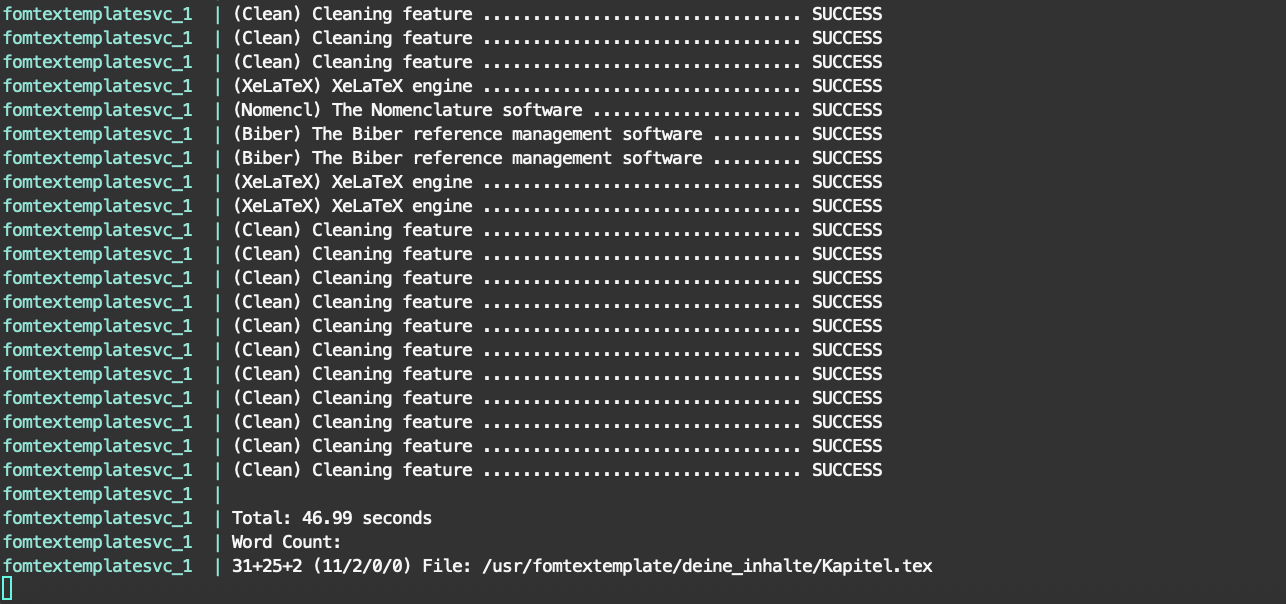
\includegraphics[width=1\textwidth]{.github/terminal}
    \captionsetup{width=1\textwidth}
    \capquelle{\cite[][200]{bsp}}\label{abb_bsp}
\end{figure}
\blindtext

\subsubsection{Tabelle}
\Blindtext\footcite[Vgl.][34]{Digitaloekonomie}\footcite[Vgl.][]{mesh}
\blinditemize
\blindtext (vgl. Tabelle \ref{tabelle_eins}).\footcite[Vgl.][511]{Tanenbaum2016}
\begin{table}[!htb]\label{tabelle_eins}
    \setlength{\arrayrulewidth}{1pt}
    \begin{threeparttable}
        \caption{Tabelle Eins}
        \begin{tabularx}{\textwidth}{|X|X|X|X|X|}
            \hline
            Spalte 1 & Spalte 2 & Spalte 3 & Spalte 4 & Spalte 5 \tabularnewline \hline
            1 & 2 & 3 & 4 & Lorem ipsum dolor sit amet \tabularnewline \hline
            1 & 2 & 3 & 4 & Lorem ipsum dolor sit amet \tabularnewline \hline
            1 & 2 & 3 & 4 & Lorem ipsum dolor sit amet \tabularnewline \hline
        \end{tabularx}
        \begin{tablenotes}[flushleft]
            \item \normalsize{Quelle: \cite[][207]{bsp}}
        \end{tablenotes}
    \end{threeparttable}
\end{table}

\subsubsection{Quelltext}
\lstinputlisting[caption={Writing Templates}\label{Templates},language=Yaml]{deine_inhalte/Quellcode/red_hat.yaml}
\captionsetup{width=1\textwidth}
\capquelle{\cite[][]{red}}\label{Red Hat} \\


\subsubsection{LaTeX-Befehle}
    \textnormal{Normale Schrift} 
    \textbullet\addspace \textbf{fette Schrift} 
    \textbullet\addspace \textit{kursive Schrift} 
    \textbullet\addspace \textsl{schiefe Schrift} 
    \textbullet\addspace \underline{unterstrichen} 
    \textbullet\addspace \texttt{Schreib\-ma\-schi\-ne} 
    \textbullet\addspace \textsf{Sans Serif} 
    \textbullet\addspace \textrm{Roman} 

\subsection{Test: Silbentrennung - Gegenüberstellung - darf nicht in den weißen Rand laufen}
Im zweiten Kapitel wird zunächst der Begriff \textit{Bring Your Own Device} (BYOD) definiert. Darauffolgend wird dargelegt welche Fokusse gesetzt werden sollen und Schlussfolgerungen gezogen, sowie eine Sicherheitsrichtlinie abgeleitet. Welche als Grundlage einer Gegenüberstellung mit etablierten Konzepten dient, sodass Strategien erörtert werden können. 

\section{Test der Ebenen und Beispieldiagramme}
\subsection{Ebene 2}
\blindtext
\begin{figure}[!htb]
  \caption{Continuous Integration Prozess}
  \captionsetup{width=1\textwidth}
  \smartdiagramset{
    border color=teal,
    uniform color list=teal!60 for 6 items,
    uniform arrow color=true,
    arrow color=gray!80,
    back arrow disabled=true
  }
  \smartdiagram[flow diagram:horizontal]{Develop \& Commit,Build,Integration,Build on Integrated Code, Integration-Tests,Packing}
  \capquelle{Eigendarstellung angelehnt an \cite[][19-20]{pathania_learning_2017}}\label{Continuous Integration Prozess}
\end{figure}
\subsection{Ebene 2.2}
\blindtext

\begin{figure}[!htb]
  \caption{Testpyramide}
  \captionsetup{width=1\textwidth}
  \begin{center}
    \begin{tikzpicture}
      \node [double arrow, draw, draw=teal, fill=teal!20, very thick, rotate=90] 
          at (-5.5,2.3) {Isolation | Integration};
      \node [double arrow, draw, draw=teal, fill=teal!20, very thick, rotate=90] 
          at (5.5,2.3) {Schnell\:\:\:\:|\:\:\:\:Langsam};
      
      \coordinate (A) at (-5,0) {};
      \coordinate (B) at (5,0) {};
      \coordinate (C) at (0,4.5) {};
      \draw[name path=AC, draw=teal, very thick] (A) -- (C);
      \draw[name path=BC, draw=teal, very thick] (B) -- (C);
      \foreach \y/\A in 
          {
            0/Unit Tests,
            1.25/Service Tests,
            2.5/UI Tests
          }
          { %0/G,1/F,2/E,3/D,4/C,5/B,6/A
            \path[name path=horiz] (A|-0,\y) -- (B|-0,\y);
            \draw[draw=teal, very thick, 
              name intersections={of=AC and horiz,by=P},
              name intersections={of=BC and horiz,by=Q}
            ] (P) -- (Q)
            node[midway,above] {\A};
          }
    \end{tikzpicture}
  \end{center}
  \capquelle{Eigendarstellung angelehnt an \cite[][311-317]{cohn_succeeding_2010}}\label{Testpyramide}
\end{figure}

\subsubsection{Ebene 3}
\blindtext
\subsubsection{Ebene 3.2}
\blindtext
\subsubsubsection{Ebene 4}
\blindtext
\subsubsubsection{Ebene 4.2}
\blindtext
\footcite[Vgl.][79]{Schelinski2019}

\section{Schluss}
\subsection{Fazit}
\blindtext (vgl. Abbildung \ref{abb_bsp}).

\subsection{Ausblick}
\blindtext

	\newpage
	\printbibliography[nottype=online,heading=bibintoc,title={Literaturverzeichnis}]
	\printbibliography[type=online,title={Internetquellen}]
	\newpage
		\newpage
\pagenumbering{gobble} % Keine Seitenzahlen mehr

%-----------------------------------
% Ehrenwörtliche Erklärung
%-----------------------------------
\section*{Ehrenwörtliche Erklärung}
Hiermit versichere ich, dass die vorliegende Arbeit von mir selbstständig und ohne unerlaubte Hilfe angefertigt worden ist, insbesondere dass ich alle Stellen, die wörtlich oder annähernd wörtlich aus Veröffentlichungen entnommen sind, durch Zitate als solche gekennzeichnet habe. Ich versichere auch, dass die von mir eingereichte schriftliche Version mit der digitalen Version übereinstimmt. Weiterhin erkläre ich, dass die Arbeit in gleicher oder ähnlicher Form noch keiner Prüfungsbehörde/Prüfungsstelle vorgelegen hat. Ich erkläre mich damit nicht einverstanden, dass die Arbeit der Öffentlichkeit zugänglich gemacht wird. Ich erkläre mich damit einverstanden, dass die Digitalversion dieser Arbeit zwecks Plagiatsprüfung auf die Server externer Anbieter hochgeladen werden darf. Die Plagiatsprüfung stellt keine Zurverfügungstellung für die Öffentlichkeit dar.


\par\medskip
\par\medskip

\vspace{5cm}

\begin{table}[H]
	\centering
	\begin{tabular*}{\textwidth}{c @{\extracolsep{\fill}} ccccc}
		München, \the\day.\the\month.\the\year
		&
		% Bilder mit transparentem Hintergrund können teils zu Problemen führen
		\includegraphics[width=0.35\textwidth]{Unterschrift}\vspace*{-0.35cm}
		\\
		\rule[0.5ex]{12em}{0.55pt} & \rule[0.5ex]{12em}{0.55pt} \\
		(Ort, Datum) & (Eigenhändige Unterschrift)
		\\
	\end{tabular*} \\
\end{table}

	\end{document}
